En la figura \ref{fig:modeloCasoUso} se muestra la estructura de información de los elementos que componen un caso de uso.

\begin{figure}[H]
	\begin{center}
		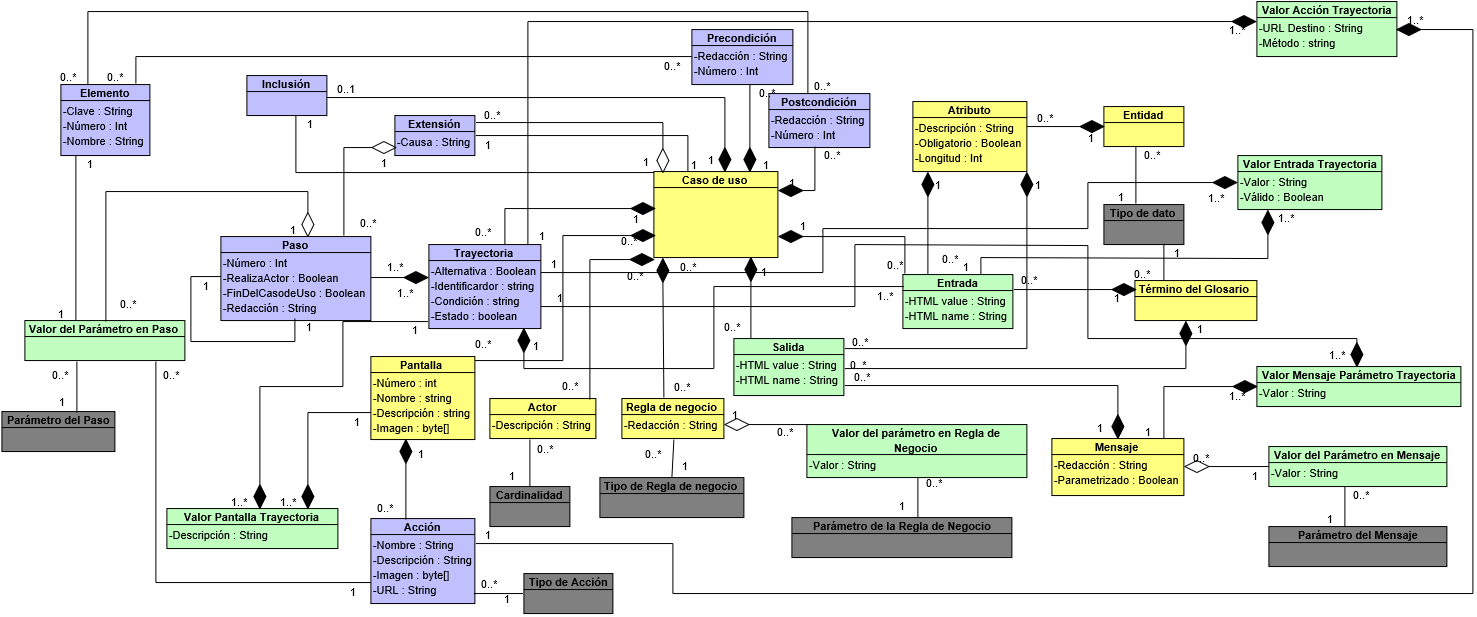
\includegraphics[angle=0,width=.95\textwidth]{images/modeloCasoUso}
		\caption{Modelo conceptual de casos de uso}
		\label{fig:modeloCasoUso}
	\end{center}
\end{figure}


\begin{BusinessEntity}{casoUso}{Caso de Uso}
	\Battr{claveCU}{Clave: }{Clave que permitirá distinguir que el elemento es un Caso de Uso. Es una palabra corta y este dato es requerido {\em (no se puede omitir)}. }
		
	\Battr{numeroCU}{Número: }{Número del Caso de Uso. Es un valor numérico entero y este dato es requerido {\em (no se puede omitir)}.}
		
	\Battr{nombreCU}{Nombre: }{Nombre que identificará al Caso de Uso. Es una frase o enunciado y este dato es requerido {\em (no se puede omitir)}.}

	\Battr{resumenCU}{Resumen: }{Breve descripción del contenido del caso de uso. Descrita en uno o más párrafos y este dato es requerido {\em (no se puede omitir)}.}
\end{BusinessEntity}

\subsubsection{Relaciones}
\begin{BusinessFact}{pantallaRelCU}{Pantalla}
	\BRitem{\textbf{Descripción: }}{Un Caso de Uso utiliza diferentes pantallas.}
	\BRitem{\textbf{Tipo: }}{\relAgregacion}
	\BRitem{\textbf{Cardinalidad: }}{Muchos a muchos}
\end{BusinessFact}

\begin{BusinessFact}{actorRelCU}{Actor}
	\BRitem{\textbf{Descripción: }}{Un Caso de Uso puede ser realizado por diferentes actores.}
	\BRitem{\textbf{Tipo: }}{\relAgregacion}
	\BRitem{\textbf{Cardinalidad: }}{Muchos a muchos}
\end{BusinessFact}

\begin{BusinessFact}{BrRelCU}{Reglas de Negocio}
	\BRitem{\textbf{Descripción: }}{Un Caso de Uso puede utilizar diferentes relgas de negocio.}
	\BRitem{\textbf{Tipo: }}{\relAgregacion}
	\BRitem{\textbf{Cardinalidad: }}{Muchos a muchos}
\end{BusinessFact}

\begin{BusinessFact}{salidaRelCU}{Salida}
	\BRitem{\textbf{Descripción: }}{Un caso de uso tiene diferentes salidas.}
	\BRitem{\textbf{Tipo: }}{\relComposicion}
	\BRitem{\textbf{Cardinalidad: }}{Uno a muchos}
\end{BusinessFact}

\begin{BusinessFact}{entradaRelCU}{Entrada}
	\BRitem{\textbf{Descripción: }}{Un caso de uso tiene diferentes entradas.}
	\BRitem{\textbf{Tipo: }}{\relComposicion}
	\BRitem{\textbf{Cardinalidad: }}{Uno a muchos}
\end{BusinessFact}

\begin{BusinessFact}{trayRelCU}{Trayectoria}
	\BRitem{\textbf{Descripción: }}{Un caso de uso se compone de trayectorias.}
	\BRitem{\textbf{Tipo: }}{\relComposicion}
	\BRitem{\textbf{Cardinalidad: }}{Uno a muchos}
\end{BusinessFact}

\begin{BusinessFact}{revRelCU}{Revisión}
	\BRitem{\textbf{Descripción: }}{Un caso de uso puede ser revisado.}
	\BRitem{\textbf{Tipo: }}{\relComposicion}
	\BRitem{\textbf{Cardinalidad: }}{Uno a muchos}
\end{BusinessFact}

\begin{BusinessFact}{extRelCU}{Extensión}
	\BRitem{\textbf{Descripción: }}{Un caso de uso puede tener puntos de extensión.}
	\BRitem{\textbf{Tipo: }}{\relComposicion}
	\BRitem{\textbf{Cardinalidad: }}{Uno a muchos}
\end{BusinessFact}

\begin{BusinessFact}{incluRelCU}{Inclusión}
	\BRitem{\textbf{Descripción: }}{Un caso de uso puede incluir otros casos de uso.}
	\BRitem{\textbf{Tipo: }}{\relComposicion}
	\BRitem{\textbf{Cardinalidad: }}{Uno a muchos}
\end{BusinessFact}

\begin{BusinessFact}{precRelCU}{Precondición}
	\BRitem{\textbf{Descripción: }}{Un caso de uso puede tener diferentes precondiciones.}
	\BRitem{\textbf{Tipo: }}{\relComposicion}
	\BRitem{\textbf{Cardinalidad: }}{Uno a muchos}
\end{BusinessFact}

\begin{BusinessFact}{postcRelCU}{Postcondición}
	\BRitem{\textbf{Descripción: }}{Un caso de uso puede tener diferentes postcondiciones.}
	\BRitem{\textbf{Tipo: }}{\relComposicion}
	\BRitem{\textbf{Cardinalidad: }}{Uno a muchos}
\end{BusinessFact}
\begin{BusinessEntity}{pantalla}{Pantalla}
	\Battr{claveIU}{Clave: }{Clave que permitirá distinguir que el elemento es una Pantalla. Es una palabra corta y este dato es \hyperlink{tRequerido}{requerido} {\em (no se puede omitir)}. }
		
	\Battr{numeroIU}{Número: }{Número de la Pantalla. Es un valor numérico entero y este dato es \hyperlink{tRequerido}{requerido} {\em (no se puede omitir)}.}
		
	\Battr{nombreIU}{Nombre: }{Nombre que identificará a la Pantalla. Es una frase o enunciado y este dato es \hyperlink{tRequerido}{requerido} {\em (no se puede omitir)}.}

	\Battr{imagenIU}{Imagen: }{Es un archivo en formato PNG o JPG. Imágen que ilustrará la interfaz gráfica del sistema. y este dato es \hyperlink{tRequerido}{requerido} {\em (no se puede omitir)}.}
	
	\Battr{patronIU}{Patrón: }{Texto que contiene la pantalla para su identificación. Es una frase o enunciado y este dato es \hyperlink{tRequerido}{requerido} {\em (no se puede omitir)}.}
\end{BusinessEntity}

\subsubsection{Relaciones}
\begin{BusinessFact}{accionRelIU}{Acción}
	\BRitem{\textbf{Descripción: }}{Una pantalla puede tener un conjunto de acciones.}
	\BRitem{\textbf{Tipo: }}{\relComposicion}
	\BRitem{\textbf{Cardinalidad: }}{Uno a muchos}
\end{BusinessFact}

\begin{BusinessEntity}{accion}{Acción}
		
	\Battr{nombreACC}{Nombre: }{Nombre que identificará a la Acción. Es una frase o enunciado y este dato es \hyperlink{tRequerido}{requerido} {\em (no se puede omitir)}.}

	\Battr{descripcionACC}{Descripción: }{Texto que describirá la Acción. Descrita en uno o más párrafos y este dato es \hyperlink{tRequerido}{requerido} {\em (no se puede omitir)}.}
	
	\Battr{imagenACC}{Imagen: }{Es un archivo en formato PNG o JPG. Imágen que ilustrará la interfaz gráfica del sistema. y este dato es \hyperlink{tRequerido}{requerido} {\em (no se puede omitir)}.}
	
	\Battr{urlACC}{URL: }{URL que determinará el destino de la acción. Es una palabra corta y este dato es \hyperlink{tRequerido}{requerido} {\em (no se puede omitir)}.}
\end{BusinessEntity}

\subsubsection{Relaciones}
\begin{BusinessFact}{pantallaRelACC}{Pantalla}
	\BRitem{\textbf{Descripción: }}{Una Acción llevará a una determinada Pantalla.}
	\BRitem{\textbf{Tipo: }}{\relAsociacion}
	\BRitem{\textbf{Cardinalidad: }}{Uno a uno}
\end{BusinessFact}

\begin{BusinessFact}{tipoRelACC}{Tipo de acción}
	\BRitem{\textbf{Descripción: }}{Una Acción es de un tipo específico.}
	\BRitem{\textbf{Tipo: }}{\relAsociacion}
	\BRitem{\textbf{Cardinalidad: }}{Muchos a uno}
\end{BusinessFact}

\begin{BusinessEntity}{actorEntidad}{Actor}
		
	\Battr{claveACT}{Clave: }{Clave que permitirá distinguir que el elemento es un Actor. Es una palabra corta y este dato
		es \hyperlink{tRequerido}{requerido} {\em (no se puede omitir)}.}

	\Battr{nombreACT}{Nombre: }{Nombre que identificará al Actor. Es una frase o enunciado y este dato es \hyperlink{tRequerido}{requerido} {\em (no se puede omitir)}.}
	
	\Battr{descripcionACT}{Descripción: }{Texto que describirá al Actor. Descrita en uno o más párrafos y este dato es \hyperlink{tRequerido}{requerido} {\em (no se puede omitir)}.}
	
	\Battr{oCardinalidadACC}{Otra cardinalidad: }{En caso de seleccionar la opción ''Otra'' como cardinalidad, este campo permitirá describirla. Es una frase o enunciado y este dato es \hyperlink{tRequerido}{requerido} {\em (no se puede omitir)}.}
\end{BusinessEntity}

\subsubsection{Relaciones}
\begin{BusinessFact}{cardinalidadRelACT}{Cardinalidad}
	\BRitem{\textbf{Descripción: }}{Un negocio cuenta con un número definido o aproximado de algún Actor.}
	\BRitem{\textbf{Tipo: }}{\relComposicion}
	\BRitem{\textbf{Cardinalidad: }}{Muchos a uno}
\end{BusinessFact}

\begin{BusinessEntity}{terminoGLSEntidad}{Término de glosario}
		
	\Battr{claveTGLS}{Clave: }{Clave que permitirá distinguir que el elemento es un Término del glosario. Es una palabra corta y este dato es \hyperlink{tRequerido}{requerido} {\em (no se puede omitir)}.}

	\Battr{nombreTGLS}{Nombre: }{Nombre que identificará al Término del glosario. Es una frase o enunciado y este dato es \hyperlink{tRequerido}{requerido} {\em (no se puede omitir)}. Este atributo debe de contener como máximo 50 caracteres. Caracteres admitidos: [A-Z] $|$ [a-z] $|$ [á-é-í-ó-ú] $|$ []}
	
	\Battr{descripcionTGLS}{Descripción: }{Texto que describirá al Término del glosario. Descrita en uno o más párrafos y este dato es \hyperlink{tRequerido}{requerido} {\em (no se puede omitir)}. Este atributo debe de contener como máximo 1000 caracteres. Caracteres admitidos: [A-Z] $|$ [a-z] $|$ [0-9] $|$ [  ] $|$ [-] $|$ [,] $|$ [á-é-í-ó-ú]}
\end{BusinessEntity}


\begin{BusinessEntity}{BREntidad}{Regla de Negocio}
		
	\Battr{claveBR}{Clave: }{Clave que permitirá distinguir que el elemento es una Regla de Negocio. Es una palabra corta y este dato es \hyperlink{tRequerido}{requerido} {\em (no se puede omitir)}.}

	\Battr{numeroBR}{Número: }{Número de Regla de Negocio. Es un valor numérico entero y este dato es \hyperlink{tRequerido}{requerido} {\em (no se puede omitir)}.}
	
	\Battr{nombreBR}{Nombre: }{Nombre que identificará a la Regla de Negocio. Es una frase o enunciado y este dato es \hyperlink{tRequerido}{requerido} {\em (no se puede omitir)}.}
	
	\Battr{redaccionBR}{Redacción: }{Redacción de la Regla de Negocio. Descrita en uno o más párrafos y este dato es \hyperlink{tRequerido}{requerido} {\em (no se puede omitir)}.}
	
	\Battr{descripcionBR}{Descripción: }{Texto que describirá al a la regla de negocio. Descrita en uno o más párrafos y este dato es \hyperlink{tOpcional}{opcional} {\em (se puede omitir)}.}
\end{BusinessEntity}

\subsubsection{Relaciones}
\begin{BusinessFact}{tipodRelBR}{Tipo de Regla de Negocio}
	\BRitem{\textbf{Descripción: }}{Una Regla de Negocio es de un tipo específico.}
	\BRitem{\textbf{Tipo: }}{\relAsociacion}
	\BRitem{\textbf{Cardinalidad: }}{Muchos a uno}
\end{BusinessFact}

\begin{BusinessFact}{operadorRelBR}{Operador}
	\BRitem{\textbf{Descripción: }}{El operador que se utiliza en una comparación de atributos.}
	\BRitem{\textbf{Tipo: }}{\relAsociacion}
	\BRitem{\textbf{Cardinalidad: }}{Muchos a uno}
\end{BusinessFact}


\begin{BusinessFact}{atributoRelBR}{Atributo}
	\BRitem{\textbf{Descripción: }}{Una regla de negocio debe especificar el atributo que hace única a una entidad.}
	\BRitem{\textbf{Tipo: }}{\relAsociacion}
	\BRitem{\textbf{Cardinalidad: }}{Muchos a uno}
\end{BusinessFact}

\begin{BusinessFact}{atributoCompRelABR}{Atributo (Comparación)}
	\BRitem{\textbf{Descripción: }}{Una regla de negocio debe especificar los atributos a comparar.}
	\BRitem{\textbf{Tipo: }}{\relAsociacion}
	\BRitem{\textbf{Cardinalidad: }}{Muchos a uno}
\end{BusinessFact}

\begin{BusinessFact}{atributoERRelABR}{Atributo (Expresión regular)}
	\BRitem{\textbf{Descripción: }}{Una regla de negocio debe especificar el atributo que se desea validar con la expresión regular.}
	\BRitem{\textbf{Tipo: }}{\relAsociacion}
	\BRitem{\textbf{Cardinalidad: }}{Muchos a uno}
\end{BusinessFact}

\begin{BusinessEntity}{MSGEntidad}{Mensaje}
		
	\Battr{claveMSG}{Clave: }{Clave que permitirá distinguir que el Elemento es un Mensaje. Es una palabra corta y este dato es \hyperlink{tRequerido}{requerido} {\em (no se puede omitir)}.}

	\Battr{numeroMSG}{Número: }{Número de Mensaje. Es un valor numérico entero y este dato es \hyperlink{tRequerido}{requerido} {\em (no se puede omitir)}.}
	
	\Battr{nombreMSG}{Nombre: }{Nombre que identificará al Mensaje. Es una frase o enunciado y este dato es \hyperlink{tRequerido}{requerido} {\em (no se puede omitir)}.}
	
	\Battr{redaccionMSG}{Redacción: }{Redacción del Mensaje. Descrita en uno o más párrafos y este dato es \hyperlink{tRequerido}{requerido} {\em (no se puede omitir)}.}
	
	\Battr{paramMSG}{Parametrizado: }{Bandera que indicará si el mensaje se encuentra parametrizado. Indica ''si'' o ''no''. y este dato es \hyperlink{tRequerido}{requerido} {\em (no se puede omitir)}.}
\end{BusinessEntity}

\subsubsection{Relaciones}
\begin{BusinessFact}{vPAramRelMSG}{Valor del parámetro en Mensaje}
	\BRitem{\textbf{Descripción: }}{Valor de los parámetros ocupados al definir el Mensaje como parametrizado.}
	\BRitem{\textbf{Tipo: }}{\relAgregacion}
	\BRitem{\textbf{Cardinalidad: }}{Uno a Muchos}
\end{BusinessFact}

\begin{BusinessEntity}{atributoEntidad}{Atributo}
	
	\Battr{nombreATR}{Nombre: }{Nombre que identificará al Atributo en la Entidad. Es una frase o enunciado y este dato es \hyperlink{tRequerido}{requerido} {\em (no se puede omitir)}. Este atributo debe de contener como máximo 50 caracteres. Caracteres admitidos: [A-Z] $|$ [a-z] $|$ [á-é-í-ó-ú] $|$ []}
	
	\Battr{descripcionATR}{Descripción: }{Texto que describirá al Atributo. Descrita en uno o más párrafos y este dato es \hyperlink{tRequerido}{requerido} {\em (no se puede omitir)}. Este atributo debe de contener como máximo 1000 caracteres. Caracteres admitidos: [A-Z] $|$ [a-z] $|$ [0-9] $|$ [  ] $|$ [-] $|$ [,] $|$ [á-é-í-ó-ú]}
	
	\Battr{obligatorioATR}{Obligatorio: }{Bandera que indicará si el Atributo es obligatorio. Indica ''si'' o ''no''. y este dato es \hyperlink{tRequerido}{requerido} {\em (no se puede omitir)}.}
	
	\Battr{longitudATR}{Longitud: }{Número que describirá la longitud máxima del Atributo. Es un valor numérico entero y este dato es \hyperlink{tRequerido}{requerido} {\em (no se puede omitir)}.}
\end{BusinessEntity}

\subsubsection{Relaciones}
\begin{BusinessFact}{tipoRelATR}{Tipo de Dato}
	\BRitem{\textbf{Descripción: }}{Un Atributo es de un tipo específico.}
	\BRitem{\textbf{Tipo: }}{\relAsociacion}
	\BRitem{\textbf{Cardinalidad: }}{Muchos a uno}
\end{BusinessFact}

\begin{BusinessEntity}{entidadEntidad}{Entidad}
		
	\Battr{claveEntidad}{Clave: }{Clave que permitirá distinguir que el elemento es una Entidad. Es una palabra corta y este dato es \hyperlink{tRequerido}{requerido} {\em (no se puede omitir)}.}

	\Battr{numeroEntidad}{Número: }{Número de Entidad. Es un valor numérico entero y este dato es \hyperlink{tRequerido}{requerido} {\em (no se puede omitir)}.}
	
	\Battr{nombreEntidad}{Nombre: }{Nombre que identificará a la Entidad. Es una frase o enunciado y este dato es \hyperlink{tRequerido}{requerido} {\em (no se puede omitir)}.}
\end{BusinessEntity}

\subsubsection{Relaciones}
\begin{BusinessFact}{atributoRelEntidad}{Atributo}
	\BRitem{\textbf{Descripción: }}{Una Entidad está compuesta por un conjunto de atributos.}
	\BRitem{\textbf{Tipo: }}{\relComposicion}
	\BRitem{\textbf{Cardinalidad: }}{Uno a muchos}
\end{BusinessFact}
\begin{BusinessEntity}{entidadTray}{Trayectoria}
		
	\Battr{alternativaTray}{Alternativa: }{Bandera que especifica si la Trayectoria es alternativa o principal. Indica ''si'' o ''no'' y este dato es \hyperlink{tRequerido}{requerido} {\em (no se puede omitir)}.}
	
	\Battr{nombreTray}{Clave: }{Nombre o clave que identificará a la Trayectroria. Es una frase o enunciado y este dato es \hyperlink{tRequerido}{requerido} {\em (no se puede omitir)}.}
	
	\Battr{condicionTray}{Condición: }{Texto que determina la circunstancia con la que se ejecuta la Trayectoria en caso de ser alternativa. Es una frase o enunciado y este dato es \hyperlink{tRequerido}{requerido} {\em (no se puede omitir)}.}
	
	\Battr{finTray}{Fin del Caso de Uso: }{Bandera que especifica si la Trayectoria concluye el Caso de uso. Indica ''si'' o ''no'' y este dato es \hyperlink{tRequerido}{requerido} {\em (no se puede omitir)}.}
\end{BusinessEntity}

\subsubsection{Relaciones}
\begin{BusinessFact}{pasoRelTray}{Paso}
	\BRitem{\textbf{Descripción: }}{Una trayectoria está compuesta por un conjunto de pasos.}
	\BRitem{\textbf{Tipo: }}{\relComposicion}
	\BRitem{\textbf{Cardinalidad: }}{Uno a muchos}
\end{BusinessFact}
\begin{BusinessEntity}{entidadPaso}{Paso}
		
	\Battr{numeroPaso}{Número: }{Número del paso en la Trayectoria. Es un valor numérico entero y este dato es \hyperlink{tRequerido}{requerido} {\em (no se puede omitir)}.}
	
	\Battr{realizaPaso}{Realiza: }{Badera que especifica quién realiza el paso, el Actor o el Sistema. Es una palabra corta y este dato es \hyperlink{tRequerido}{requerido} {\em (no se puede omitir)}.}
	
	\Battr{condicionTray}{Condición: }{Texto que determina la circunstancia con la que se ejecuta la Trayectoria en caso de ser alternativa. Es una frase o enunciado y este dato es \hyperlink{tRequerido}{requerido} {\em (no se puede omitir)}.}
	
	\Battr{redaccionPaso}{Redacción: }{Redacción del Paso. Es una frase o enunciado y este dato es \hyperlink{tRequerido}{requerido} {\em (no se puede omitir)}.}
\end{BusinessEntity}

\subsubsection{Relaciones}
\begin{BusinessFact}{pasoRelPaso}{Paso}
	\BRitem{\textbf{Descripción: }}{Un Paso de la Trayectoria puede continuar con otro Paso de alguna Trayectoria.}
	\BRitem{\textbf{Tipo: }}{\relComposicion}
	\BRitem{\textbf{Cardinalidad: }}{Uno a uno}
\end{BusinessFact}

\begin{BusinessFact}{vParamRelPaso}{Valor del Parámetro en Paso}
	\BRitem{\textbf{Descripción: }}{Valor de los parámetros ocupados al definir el Paso.}
	\BRitem{\textbf{Tipo: }}{\relAgregacion}
	\BRitem{\textbf{Cardinalidad: }}{Uno a muchos}
\end{BusinessFact}
\begin{BusinessEntity}{entidadValorParamPaso}{Valor del Parámetro en Paso}
		
	\item Esta entidad no cuenta con atributos y únicamente sirve para ilustrar que el Paso cuenta con valores determinados por las relaciones de esta entidad.
	
\end{BusinessEntity}

\subsubsection{Relaciones}
\begin{BusinessFact}{elementoRelValorParamPaso}{Elemento}
	\BRitem{\textbf{Descripción: }}{El valor utilizado en el Paso corresponde a un Elemento.}
	\BRitem{\textbf{Tipo: }}{\relAsociacion}
	\BRitem{\textbf{Cardinalidad: }}{Muchos a uno}
\end{BusinessFact}

\begin{BusinessFact}{accionRelValorParamPaso}{Acción}
	\BRitem{\textbf{Descripción: }}{El valor utilizado en el Paso corresponde a una Acción.}
	\BRitem{\textbf{Tipo: }}{\relAsociacion}
	\BRitem{\textbf{Cardinalidad: }}{Muchos a uno}
\end{BusinessFact}

\begin{BusinessFact}{tipoRelValorParamPaso}{Tipo}
	\BRitem{\textbf{Descripción: }}{El valor utilizado en el Paso es de un tipo específico.}
	\BRitem{\textbf{Tipo: }}{\relAsociacion}
	\BRitem{\textbf{Cardinalidad: }}{Muchos a uno}
\end{BusinessFact}
\begin{BusinessEntity}{revisionEntidad}{Revisión}
	
	\Battr{observacionRevision}{Observaciones: }{Descripción de las correcciones que necesita el caso de uso. Descrita en uno o más párrafos y este dato es \hyperlink{tRequerido}{requerido} {\em (no se puede omitir)}.}
	
	\Battr{seccionRevision}{Sección: }{Es la sección sobre la que se hacen las correcciones. Es una frase o enunciado y este dato es \hyperlink{tRequerido}{requerido} {\em (no se puede omitir)}.}
\end{BusinessEntity}

\subsubsection{Relaciones}
\begin{BusinessFact}{actualizacionRelRevision}{Actualización}
	\BRitem{\textbf{Descripción: }}{El analista realiza una revisión de la Actualización.}
	\BRitem{\textbf{Tipo: }}{\relAsociacion}
	\BRitem{\textbf{Cardinalidad: }}{Muchos a uno}
\end{BusinessFact}
\begin{BusinessEntity}{entidadExtension}{Extensión}
		
	\Battr{observacionRevision}{Número: }{Texto que describe la razón por la que se extiende a otro Caso de Uso. Es una frase o enunciado y este dato es \hyperlink{tRequerido}{requerido} {\em (no se puede omitir)}.}.
\end{BusinessEntity}

\subsubsection{Relaciones}
\begin{BusinessFact}{pasoRelExtension}{Paso}
	\BRitem{\textbf{Descripción: }}{El punto de extensión ocurre en alguna región de la Trayectoria.}
	\BRitem{\textbf{Tipo: }}{\relAsociacion}
	\BRitem{\textbf{Cardinalidad: }}{Uno a muchos}
\end{BusinessFact}

\begin{BusinessFact}{CURelExtension}{Caso de Uso}
	\BRitem{\textbf{Descripción: }}{Un punto de extensión extiende a un Caso de Uso.}
	\BRitem{\textbf{Tipo: }}{\relAsociacion}
	\BRitem{\textbf{Cardinalidad: }}{Uno a uno}
\end{BusinessFact}
\begin{BusinessEntity}{entidadInclusion}{Inclusión}
		
	\item Esta entidad no cuenta con atributos y únicamente sirve para ilustrar que la Inclusión se compone por la relación con el Caso de Uso.
\end{BusinessEntity}

\subsubsection{Relaciones}

\begin{BusinessFact}{CURelInclusion}{Caso de Uso}
	\BRitem{\textbf{Descripción: }}{Una inclusión hace referencia a un Caso de Uso.}
	\BRitem{\textbf{Tipo: }}{\relAsociacion}
	\BRitem{\textbf{Cardinalidad: }}{Uno a uno}
\end{BusinessFact}
\begin{BusinessEntity}{entidadPrecondicion}{Precondición}
		
	\Battr{redaccionPrecondicion}{Redacción: }{Redacción de la Precondición. Descrita en uno o más párrafos y este dato es \hyperlink{tRequerido}{requerido} {\em (no se puede omitir)}.}
	
	\Battr{numeroPrecondicion}{Número: }{Número de la Precondición. Es un valor numérico entero y este dato es \hyperlink{tRequerido}{requerido} {\em (no se puede omitir)}.}
	
\end{BusinessEntity}

\subsubsection{Relaciones}

\begin{BusinessFact}{elementoRelPrecondicion}{Elemento}
	\BRitem{\textbf{Descripción: }}{La Precondición se encuentra constituida por diferentes elementos.}
	\BRitem{\textbf{Tipo: }}{\relAsociacion}
	\BRitem{\textbf{Cardinalidad: }}{Muchos a Muchos}
\end{BusinessFact}
\begin{BusinessEntity}{entidadPostcondicion}{Postcondición}
		
	\Battr{redaccionPostcondicion}{Redacción: }{Redacción de la Postcondición. Descrita en uno o más párrafos y este dato es \hyperlink{tRequerido}{requerido} {\em (no se puede omitir)}.}
	
	\Battr{numeroPostcondicion}{Número: }{Número de la Postcondición. Es un valor numérico entero y este dato es \hyperlink{tRequerido}{requerido} {\em (no se puede omitir)}.}
	
\end{BusinessEntity}

\subsubsection{Relaciones}

\begin{BusinessFact}{elementoRelPrecondicion}{Elemento}
	\BRitem{\textbf{Descripción: }}{La Postcondición se encuentra constituida por diferentes elementos.}
	\BRitem{\textbf{Tipo: }}{\relAsociacion}
	\BRitem{\textbf{Cardinalidad: }}{Muchos a Muchos}
\end{BusinessFact}